% "Станет проще"

\documentclass[a4paper,12pt]{article} % тип документа

% report, book

% Рисунки
\usepackage{graphicx}
\usepackage{wrapfig}

\usepackage{hyperref}
\usepackage[rgb]{xcolor}
\hypersetup{				% Гиперссылки
    colorlinks=true,       	% false: ссылки в рамках
	urlcolor=blue          % на URL
}

%  Русский язык

\usepackage[T2A]{fontenc}			% кодировка
\usepackage[utf8]{inputenc}			% кодировка исходного текста
\usepackage[english,russian]{babel}	% локализация и переносы


% Математика
\usepackage{amsmath,amsfonts,amssymb,amsthm,mathtools} 


\usepackage{wasysym}

%Заговолок
\author{Дерзай знать}
\title{Общие принципы и математика в \LaTeX{}}
\date{\today}


\begin{document} % начало документа

\maketitle

\tableofcontents

\newpage

Наша первая строчка.\\[2cm]
Вторая \hspace{20pt} строчка.

Важное можно выделить \textbf{жирным}

Эстеты могут воспользоваться \textit{курсивом}

Прагматичные могут \underline{подчеркнуть}

Можно даже \fbox{в рамочку}

Дефис -- не тире.

Кавычки это не Shift+2. Кавычки это <<так>>

\section{Мир формул}

Наша первая формула $100+100=200$, ага.

\[ 100+100=200 \]

\begin{equation}\label{pifagor}
a^2+b^2=c^2
\end{equation}

Теорему Пифагора \eqref{pifagor} вы знаете с 8 класса\footnote{Определенно знали}. Эта теорема упоминается на странице \pageref{pifagor}.

\subsection{Дроби}

$\frac{1}{3}+\frac{1}{3}=\frac{2}{3}$. Вот вам и дроби\footnote{А это с пятого класса.}. {\scriptsize Так некрасиво.} {\Large Красиво так}:

\[ \frac{1}{3}+\frac{1}{3}=\frac{2}{3} \]


\subsection{Скобки}

\[ (2+3)\cdot 5=25 \]

\[ \left[\frac{4}{2}+3\right]\cdot 5=25 \]

\[ \{2+3\}\cdot 5=25 \]

\subsection{Индексы}

\[ m_1, m_{12}, c^2, c^{22} \]

\subsection{Стандартные функции}

\[ \sin x=0 \]
\[ \arctg x=\sqrt[5]{3} \]
\[ \log_{x-1}{(x^2-3x-4)}\geqslant 2 \]
\[ \lg 10=\ln e \]

$  $\subsection{Функции покрупнее}

$\sum_{i=1}^{n}a_i+b_i$

\[ \sum_{i=1}^{n}a_i+b_i \]

$I=\int r^2dm$

\[I=\int r^2dm \]

\[I=\int_{0}^{1} r^2dm \]

\[I=\int\limits_{0}^{1} r^2dm \]

\subsection{Символы}

\[2\times 2\neq 5 \]

\[x \cap y,  x \cup y\]

\[x\in (-\infty; 0),\]

\[ \triangle ABC = \triangle A_1B_1C_1 \Rightarrow \angle A= \angle A_1\]

\smiley


\newpage

\begin{center}
Вторая часть! Ура!!!
\end{center}

\begin{flushright}
Мы надеемся, что вы уже активно готовитесь к сдаче коллоквиума и вовсю смотрите программу <<Мама, я Гейне!>>. Потому что если нет, то Таежный брат Владислав вас найдет. Так что вперед.
\end{flushright}

\begin{itemize}
\item Общие вопросы;
\item Работа с текстом;
\item Математика
\begin{itemize}
\item Дроби;
\item Скобки;
\item Многое другое
\end{itemize}
\end{itemize}

\begin{enumerate}


\item Общие вопросы;
\item Математика
\item Работа с текстом;

\begin{itemize}
\item Дроби;
\item Скобки;
\item Многое другое
\end{itemize}
\end{enumerate}


\subsection{Диакритические знаки}

\[ \dot{x}=0, \]
\[ \tilde{a}=\overline{bcde}, \]
\[ \overrightarrow{a} (0,3,4), \]
\[ \underbrace{1+2+3+\dots+n}_{n}=N, \]
\[ (x-1)(x+1)>0 \stackrel{x>0}{\Longleftrightarrow} x-1>0, \]


\subsection{Буквы других алфавитов и математические шрифты}

\[ \sin \alpha = 0, \]
\[ \omega = \frac{2\pi}{T}, \]
\[ \epsilon, \varepsilon, \varphi \]
\[ \overrightarrow{a}=\mathbf{a}, \]
\[ x\in R, \]
\[ x\in \mathbb{R}, \]
\[ m_{\text{груза}}= 15~\text{кг} \]


\subsection{Матрицы}

\[ \begin{pmatrix}
a_{11} & a_{12} & a_{13} \\
a_{21} & a_{22} & a_{23}
\end{pmatrix} \]

\[ \begin{bmatrix}
a_{11} & a_{12} & a_{13} \\
a_{21} & a_{22} & a_{23}
\end{bmatrix} \]

\[ \begin{Vmatrix}
a_{11} & a_{12} & a_{13} \\
a_{21} & a_{22} & a_{23}
\end{Vmatrix} \]

\[ \begin{vmatrix}
a_{11} & a_{12} & a_{13} \\
a_{21} & a_{22} & a_{23} \\
a_{31} & a_{32} & a_{33}
\end{vmatrix} \]

\section{Группировка формул}

\begin{equation}
\begin{aligned}
2 &\times a=4,\\
-3 &\times b = 6,\\
-100 &\times c = 110.
\end{aligned}
\end{equation}

\begin{equation}
\begin{aligned}
2 &\times a=4, & &3 \times x=11,\\
-3 &\times b = 6, & &-123 \times y =123,\\
-100 &\times c = 110, & &-100z=0. 
\end{aligned}
\end{equation}

\[  \left\{
\begin{aligned}
&2 \times a=4,\\
&-3 \times b = 6,\\
&-100 \times c = 110.
\end{aligned} \right.
\]

\[  \left[
\begin{aligned}
&2 \times a=4,\\
&-3 \times b = 6,\\
&-100 \times c = 110.
\end{aligned} \right.
\]

\[  \left.
\begin{aligned}
2 \times a=4&\\
-3 \times b = 6&\\
-100 \times c = 110&
\end{aligned} \right\} \Rightarrow -6ab=24
\]

\section{Картинки}


\includegraphics[scale=0.3]{dz_rastr}


\includegraphics[width=2cm]{dz_rastr}


\includegraphics[height=4cm]{dz_rastr}


\includegraphics[width=0.5\textwidth]{dz_rastr}

\begin{figure}[h!]
\begin{center}

\includegraphics[width=0.5\textwidth]{dz_rastr}
\end{center}
\caption{Дерзай знать!} \label{dz1}
\end{figure}

Наш логотип представлен на рисунке \ref{dz1}


\begin{figure}[h!]
\begin{center}

\includegraphics[width=0.4\textwidth]{dz_vec}
\end{center}
\caption{Дерзай знать!} \label{dz2}
\end{figure}

Наш векторный логотип представлен на рисунке \ref{dz2}

% растровые (jpg, png,...)
% векторные (pdf, eps, cdr,...)

\newpage

\section{Таблицы}

\begin{table}
\caption{Погрешности}
\begin{tabular}{|c|c|rp{5cm}|}
\hline 
\multicolumn{3}{|c|}{Погрешности} &  Подробнейший комментарий нашего дорогого Таежного брата\\ 
\hline \hline 
Систематическая & Случайная & Итог & \\ 

$\sigma_1=0,04$ & $\sigma_2=0,03$ & $\sigma=0,05$ & \\ 
\hline 
\end{tabular} 
\end{table}

\section{Картинки и таблицы в тексте}
\begin{wrapfigure}{l}{6cm}
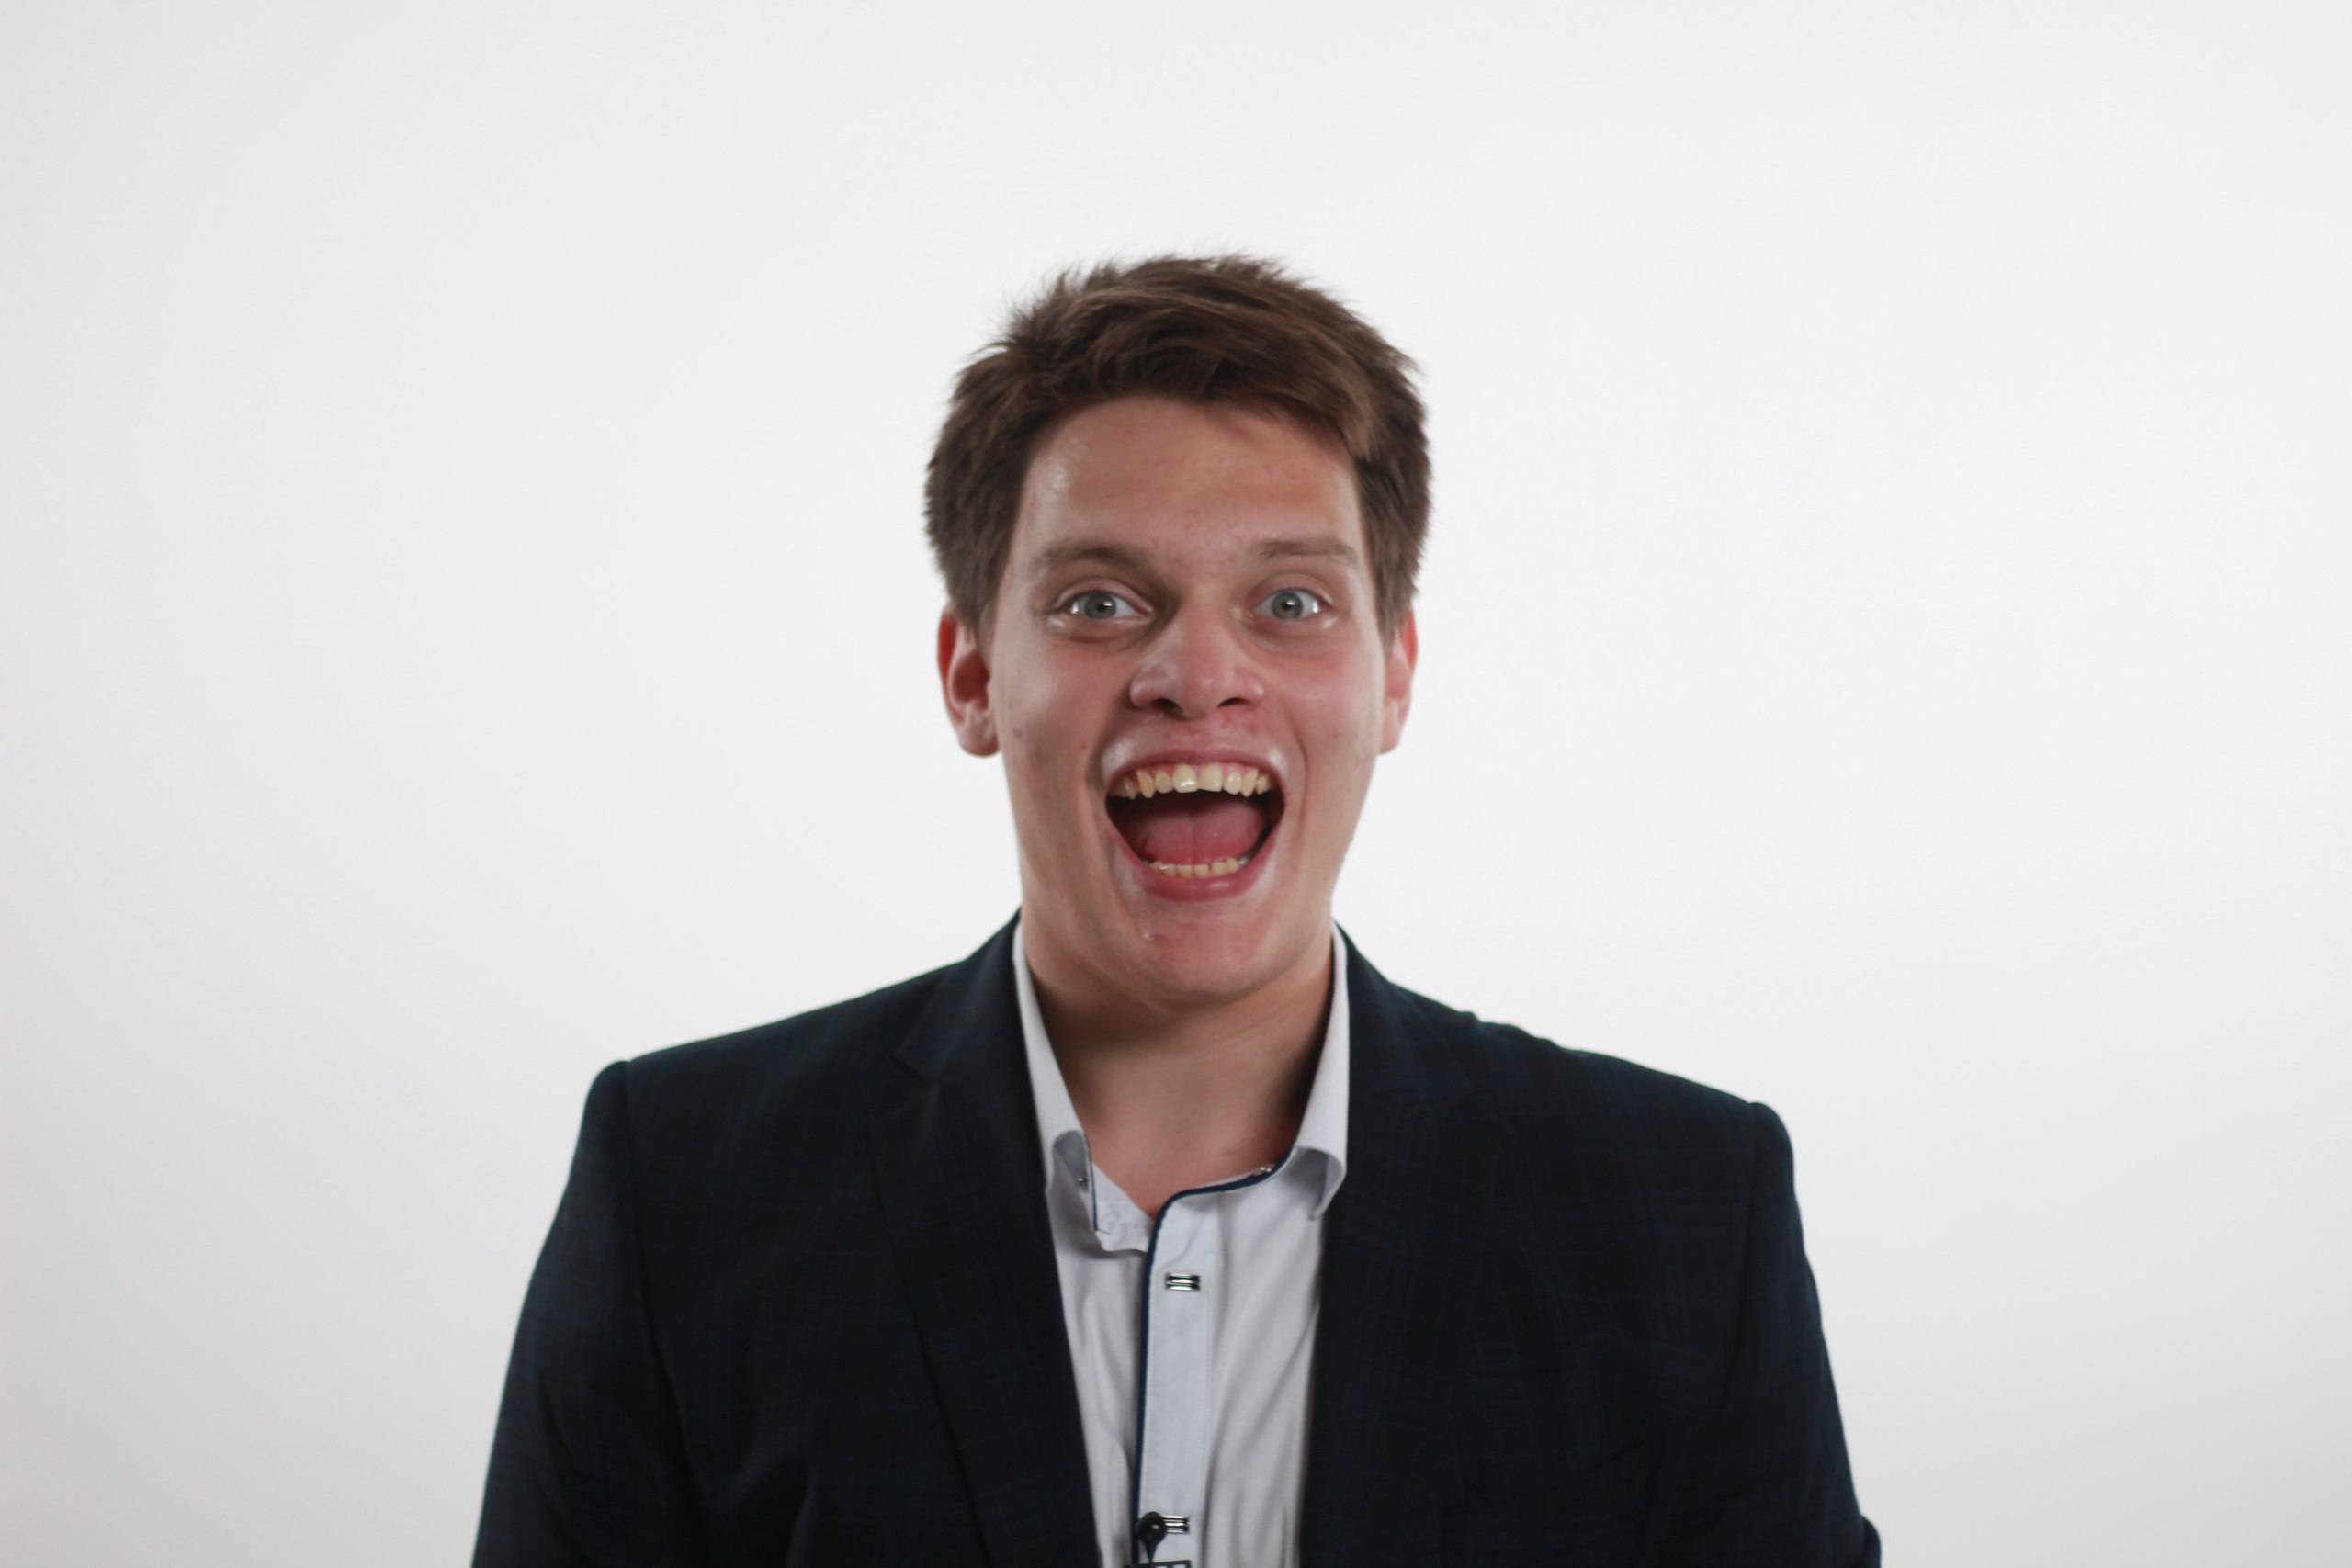
\includegraphics[width=6cm]{brat}
\caption{Таежный брат}
\end{wrapfigure} Юрлов Владислав Витальевич, дата рождения: 31.10.1997, паспорт: серия 2434 номер 1212121, проживает по адресу Москва, улица Тверская, дом 1, кв 789, прописан по адресу: США, Нью-Йорк, Бродвей, дом 156, квартира 457. Судимостей не имеет, справка о состоянии здоровья предоставлена. Подано заявление о приеме на работу в качестве совместителя, на должность ведущего <<Мама, я Гейне!>> Основное место работы: ведущий консультант Tesla Motors, США. Прилагаются рекомендации о приеме на работу от: Илон Маск, Дональд Трамп. 

\begin{wraptable}{r}{3cm}
\begin{tabular}{|c|c|c|}
\hline 
$A$ & $B$ & $C$ \\ 
\hline 
1 & 2 & 3 \\ 
\hline 
\end{tabular} 
\caption{Бесполезная таблица}
\end{wraptable} Бесполезная таблица. Бесполезная таблица. Бесполезная таблица. Бесполезная таблица. Бесполезная таблица. Бесполезная таблица. Бесполезная таблица. Бесполезная таблица. Бесполезная таблица. Бесполезная таблица. Бесполезная таблица. Бесполезная таблица. 

\listoffigures
\listoftables

\section{Ссылки}

\begin{itemize}
\item С.М. Львовский. \LaTeX : подробное описание;
\item Топовый \href{https://www.coursera.org/learn/latex}{курс} от ВШЭ.
\end{itemize}


\end{document} % конец документа